Cobit deriva dal COSO.

\subsubsection{Monitoring} 
Quando vedete una freccia è circolare bisogna pensare al \textbf{PDCA} (Plan Do 
Check Act). Infatti tutti i progetti sono ormai circolari.  
\emph{Kaizen} parola giapponese che vuol dire ``miglioramento continuo''
Scostamento tra valore atteso e valore ottenuto. Quando si vede che c'è un delta 
 si cerca di operare per migliorarlo.
Una volta raggiunto l'obiettivo, bisogna migliorare.

\begin{itemize}
\item Monitorare e valutare la performance dell'IT.
\item Compliance:
SRL (Società responsabilità limitata) dopo il caso ERON? se non si intraprendono 
le attività proattive per quanto riguarda la sicurezza si hanno conseguenze 
legali.
Sulla nuova normativa di privacy se l'azienda non intraprenderà le procedure 
adeguate per preservare la privacy, avrà delle multe fino al 5\% del fatturato e 
la possibilità di andare a processo.
\item 
\item 
\end{itemize}

\subsubsection{SSE-CMM: System Security Eng -- Capability Maturity Model}
Modelli di maturità. Questa categorizzazione si applica a tutto. Nata per 
l'ingegneria del Software.
La maturità è la capacità di governare i processi. Se si riesce anche a mettere 
in pratica il miglioramento continuo si è a livelli alti.

Gli investitori saranno più portati a investire in aziende hanno un CMM alto 
rispetto a uno basso, in quanto quelle basse (dallo stage 2 in giù) sono legate 
al lato ``umano''. Essere a livelli alti è anche un vantaggio che si può portare 
al mercato.

Grazie a questo è possibile mettere in piedi un sistema di miglioramento 
continuo.

\begin{figure}[h!]
        \begin{center}
                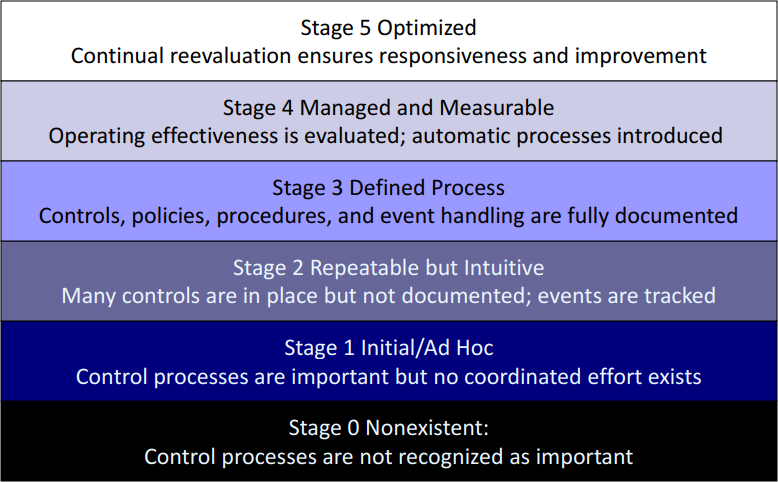
\includegraphics[scale=2.0]{res/img/maturity_level}
        \end{center}
        \caption{I 5 livelli del Capability Maturity Model (CMM).}
        \label{fig:cmm:levels}
\end{figure}

Se i controlli non sono documentati non si sa come possono essere migliorati, 
valutarli ecc\dots
(Dal Livello 4 in su) Automatizzazione dei processi di controllo permettono un 
risparmio sul TCO (Total Cost of Ownership).
\textbf{I livelli sono molto importanti}.


\subsubsection{Standard di sicurezza}

ISO 27001 e il COBIT sono gli standard di sicurezza di base. La\textit{gap 
analysis} ci aiuta a vedere dove sono presenti differenze da colmare.

\begin{figure}[h!]
        \begin{center}
                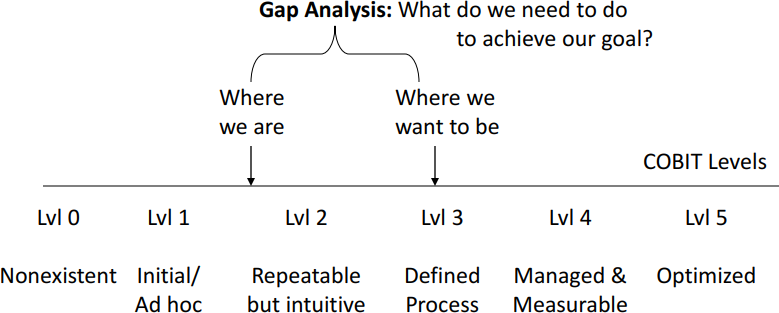
\includegraphics[scale=2.0]{res/img/security_standard}
        \end{center}
        \caption{I 5 livelli del Capability Maturity Model (CMM) e il
        loro rapporto con un programma di sicurezza.}
        \label{fig:}
\end{figure}


\paragraph{Livello 0}


Al livello iniziale si è come un pompiere, che si corre a destra e a sinistra a 
risolvere eventuali problemi.

\paragraph{Livello 1}

I problemi di sicurezza sono trattati in maniera reattiva, ovvero si reagisce 
alla minaccia (portando prima o poi l'attacco a vincere). Non ci sono piani di 
contingenza\footnote{I piani di contingenza sono dei piani che dettano le azioni 
da compiere in caso si verificano delle situazioni d'emergenza.}. Il lavoro 
viene compiuto sempre \textit{ad hoc}.

\paragraph{Livello 2 - Pianficazione}

Gli eventi sono tracciati, ma si segue una pianificazione 
"personalizzata"\footnote{Vedi come esempio la morte nera.}.

\paragraph{Livello 3}
I processi sono standardizzati le persone sanno cosa fare riusciamo a tracciare 
la performance. 



Con il livello 3 è possibile sopravvivere ad un livello negativo forte.






Quando vengono assunti i nuovi dipendenti fanno corsi, ecc.








\paragraph{Livello 4 - Metriche}


Il livello 4 è tutto scritto e documentato, e sono presenti politiche, 
procedure, standard e \textit{guidelines}. Tutto dev'essere documentato (e c'è 
tanta carta quindi).

% Speck


\subparagraph{Esempi di policy}

\begin{itemize}
\item Rischi
\item Monitoraggio e metriche
\item Risposta all'incidente
\item Business continuity e disaster recovery plan
\end{itemize}

Nota: una cattiva \textit{policy} fa riferimento alla tecnologia. Le 
\textit{policy} sono solamente linee guida.

\subsubparagraph*{Definizioni di qualità}

\begin{itemize}
\item Quality assurance 
\item Quality control è piú semplice si può vaidare con dei test.
\end{itemize}





\subsubparagraph{Metriche}

Senza metriche è impossibile migliorarsi perché non si sa cosa succede.
Senza metriche quantitative si lascia spazio alla soggettività.

\subsubparagraph*{Metriche operazionali}

Le metriche di tipo operazionali per esempio includono metriche su come eseguire 
un corretto \textit{patching} dei sistemi.


\begin{figure}[h!]
        \begin{center}
                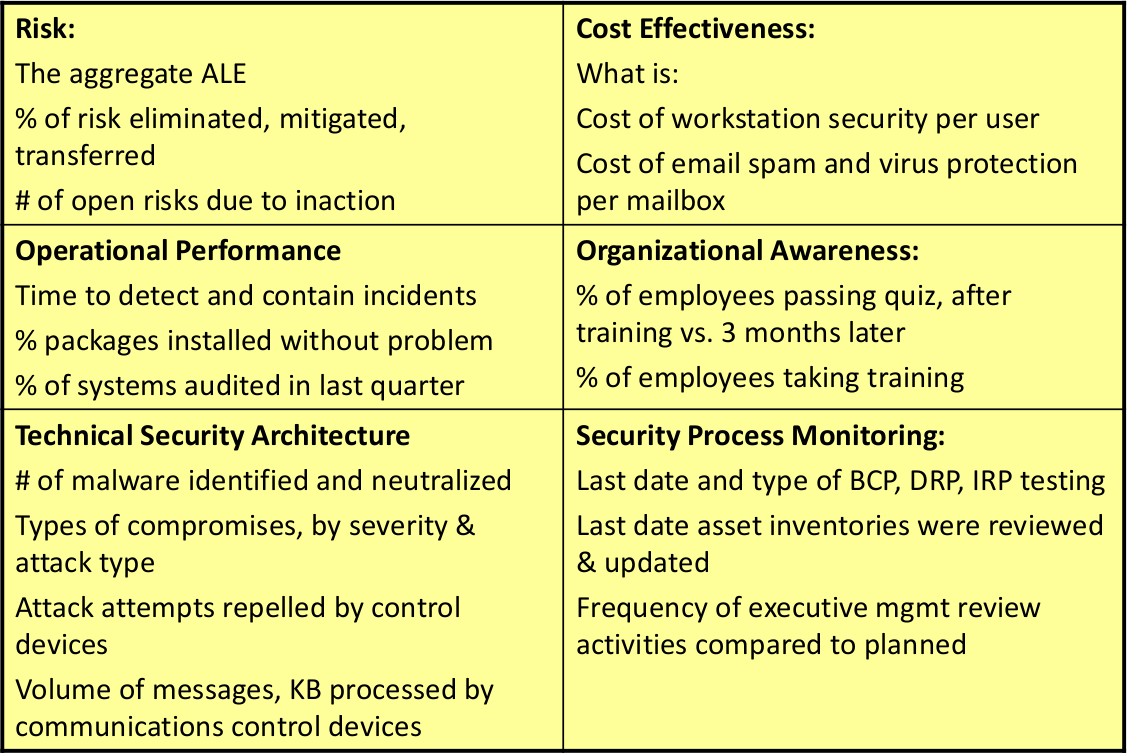
\includegraphics[scale=1.5]{res/img/metriche}
        \end{center}
        \caption{Esempi di metriche per un'azienda.}
        
\end{figure}

Confrontare le metriche con quelle di altre aziende permette di capire quanto 
siamo un possibile \textit{target} per possibile attaccanti.

\subsubparagraph*{Metriche di tipo strategico}

Sono i piani legati al rischio, come il \textit{disaster recovery}.
Il rapporto di audit è una metrica importantissima perché fa capire come lavora 
l'azienda e l'auditor.

\subsubparagraph{Compliance interna}


La \textit{compliance} sono fotografie che in qualche modo catturano la realtà 
in qualche momento. Compliance e errore interno sono dati importanti perché 
fanno capire all'azienda quanto è allineata con gli obiettivi strategici che si 
è prefissata.


\paragraph{Livello 5 - Ottimizzazione}

Miglioramento continuo e ottimizzazione. Plan Do check act.
Si svolgono anche azioni proattive. Funzione strategica "new tehnologies" come 
le nuove tecnologie possono essere fless per gli obiettivi aziendali. 
Prima avere un cambio tecnologico di fondo è raro mentre oggi ogni 3 anni. Chi 
prende la tecnologia e la incoropora si prende la fetta di mercato. Tecnologia 
disruttiva?.

%         /\
%        /  \
%        \/\/
%         ~|
%        !~~-!
%        |` ,!
%        |'` |
%        |   |
%        |   |
%        |   |
%        |   |
%        |   |
% _______|___|_______
% \                 /
%  \_______________/



Le grande società fanno \textit{scouting} di nuove tecnologie. Il vantaggio di 
essere un'azienda piccola è che si può essere aggressivi e investire. Questo 
aiuta il movimento economico. Questo ci dice che aziende come Google non ci 
saranno per sempre. Con il cambiamento tecnologico non si è ancora capito a dove 
possono portare. Un'altra area importante è l'intelligenza artificiale legata 
alla sicurezza.


\subsubsection{Esercizi}

Gli esercizi sono disponibili in \ref{esSM:COBIT}

\chapter{Policy and Governance}
\label{PG}

\section{Coorporate governance}

È la leadership che consente di arrivare ad avere valore per gli stakeholders.
L'IT governance sia assicura del corretto alligneamento dell'IT con gli 
obiettivi aziendali. dell'azienda.



\section{Strategic Planning Proccess}
\label{PG:SPP}

Oggi come oggi una pianificazione strategica nell'IT è in 3 anni, in quanto tra 
5 anni nessuno sa cosa ci sarà. Quindi la lunghezza dei piani si è accorciata, 
specialmente nel settore informatico in quanto la pressione tecnologica è 
altissima. Questa pianificazione è destinata ad accorciarsi grazie 
all'intelligenza artificiale, che aiuterà gli umani a prendere decisioni.
